\documentclass[main]{subfiles}


\begin{document}
\newpage
\section{Neuromorphic Systems 1}

\subsection{History and motivation}

\subsubsection{History}
Neuromorphic Engineering (NE) Neuromorphic engineering is a relatively young field that attempts to build physical realizations of biologically realistic models of neural systems using electronic circuits implemented in very large scale integration technology. The concept was coined by Carver Mead in the late 1980s. Carver Mead together with John Hopfield and Richard Feynmann started the Physics of Computation course at Caltech, which later transformed to the fully-flagged Phd/MSc program called "Computation and Neural Systems". Notable alumni are INI professors like Tobi Delbruck, Shi-Chi Liu and Giacomo Indiveri. Carver Mead also coined Moore's Law:  the number of transistors in a dense integrated circuit doubles about every two years.

\subsubsection{Physical comparisons: channel vs. transistor}

NE is possible because the physics of voltage activated membrane channels and transistors are closely related. When MOSFETs are operated in the weak-inversion regime (sub-threshold), the main mechanism of carrier transport is that of diffusion, as it is for ions flowing through proteic channels across neuron membranes:

\begin{itemize}
    \item $K^+$ conductance of cell membrane increases exponentially with the membrane voltage, until it approaches saturation at the maximal opening of the channel.
    \item Drain-to-Source Current ($I_{DS}$) flowing through a MOS transistors increases exponentially with the Gate-to-Source Voltage ($V_{GS}$) below a specific "threshold" voltage and quadratically above this value.
\end{itemize}{}

%
\begin{figure}[h]
    \centering
    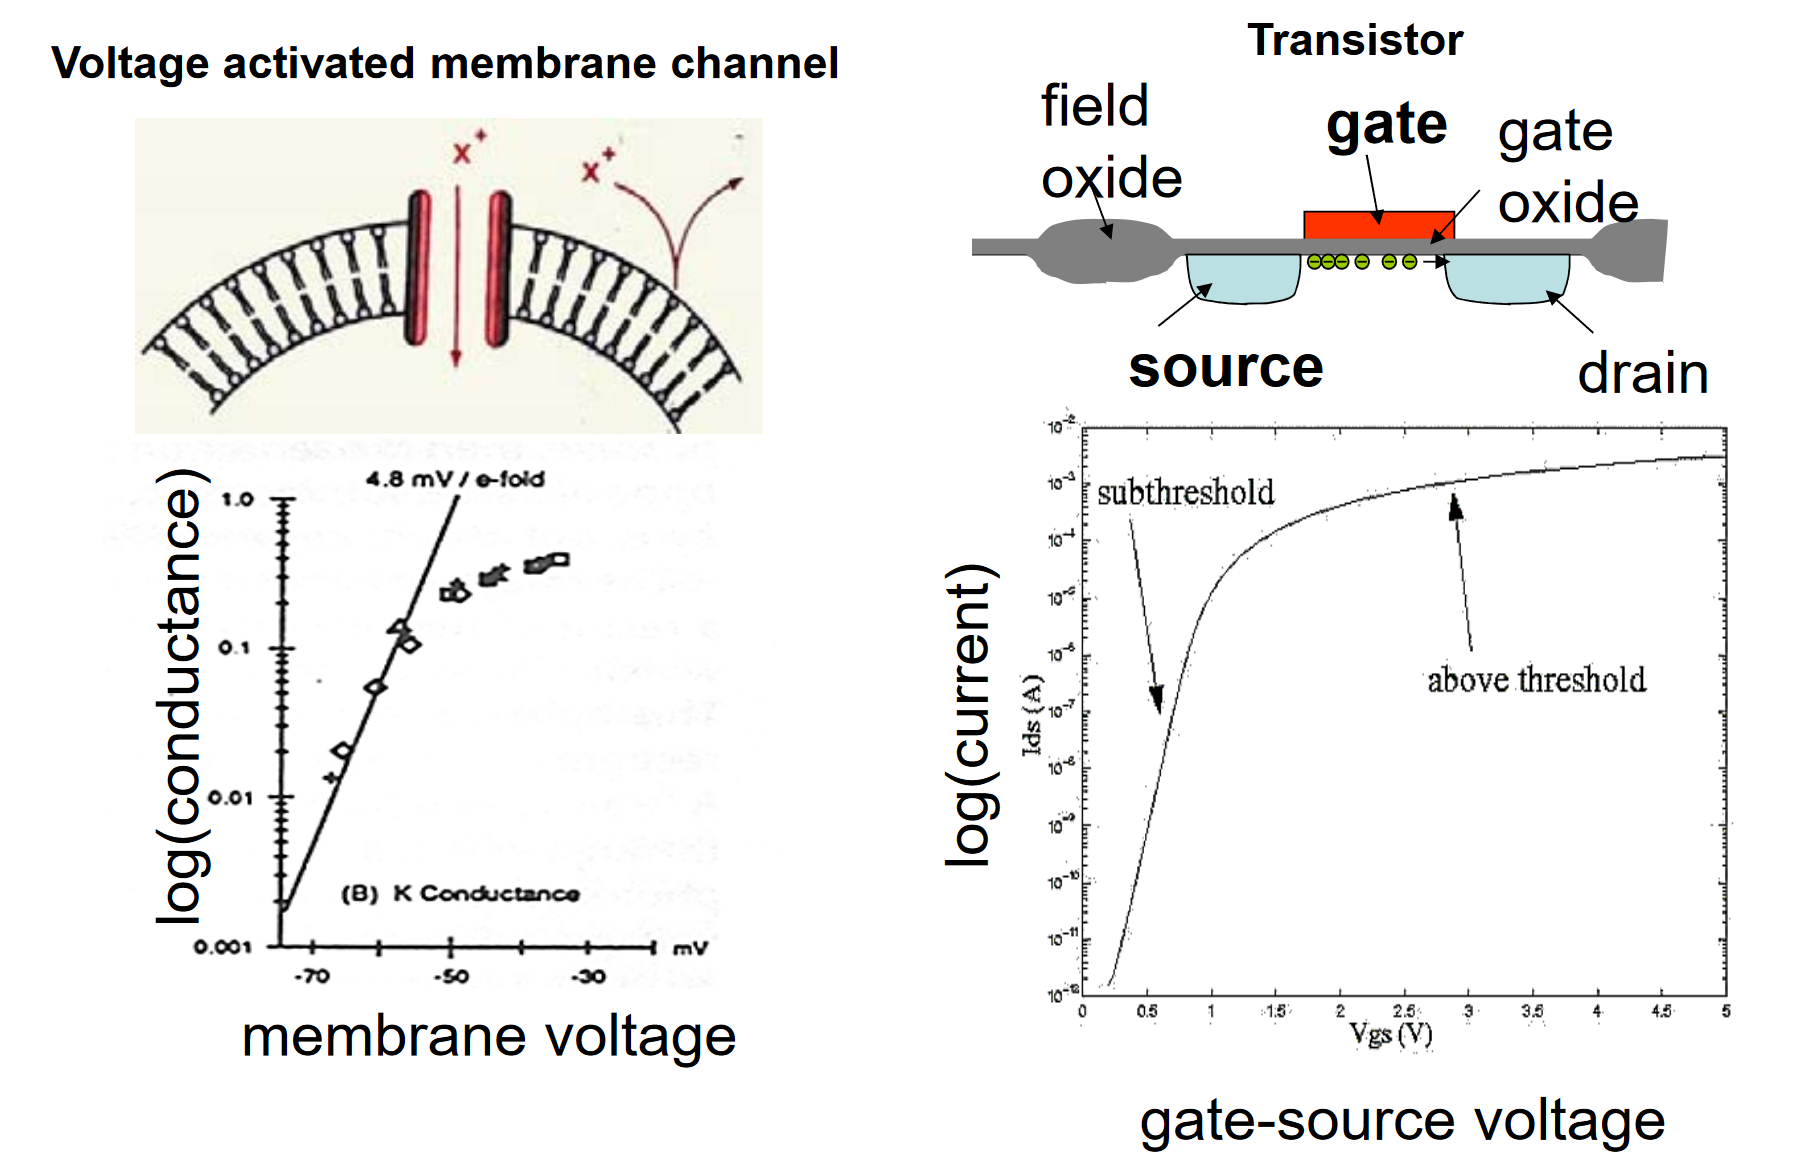
\includegraphics[width=0.8\linewidth]{11_NeuromorphicSystems1/figures/mem_vs_transist.PNG}
    \caption{Comparing a voltage activated membrane channel to the MOS transistor.}
    \label{fig:MEMvsTRANS}
\end{figure}
%

\subsubsection{Physical comparisons: brain vs. computer}
Even though conventional computation powered by silicon has seen immense gains in the past decades, as predicted by Moore's law, natural computation is still at least a million times more power efficient.

Some notable differences between brain-natural and artificial computation are presented below:

\begin{table}[h]
\begin{tabular}{|c|c|}
\hline
\textbf{Artificial Computation}         & \textbf{Brain}                                \\ \hline
Fast clocked system (GHz)               & Self-timed, data-driven (0.1 Hz to tens kHz)  \\ \hline
Bit-perfect deterministic logical state & Synapses are stochastic                       \\ \hline
Memory distant to computation           & Memory local to computation                   \\ \hline
High-bit resolution                     & Low-bit resolution with neurons as quantizers \\ \hline
\end{tabular}
\end{table}

\subsubsection{Physical comparisons: cell vs. ALU}
When looking at individual neuronal cells structurally we can define a set of computational steps executed by each main components:

\begin{itemize}
    \item \textbf{Channels} execute a form of multiplication as observed in Figure \ref{fig:MEMvsTRANS}.
    \item \textbf{Synapses} host populations of channels which open at the arrival of a PSP. The effect of each channel in the population is summed up, making the synapse behave like a Multiply-Accumulate unit.
    \item \textbf{Cell membrane} hosts complementary channels which can both increase the membrane voltage or decrease it.
    \item \textbf{Dendrites} connect to pre-synaptic neurons through both excitatory and inhibitory synapses, leading to analog additions and subtractions being executed at the level of single dendrites.
    \item \textbf{Dendritic trees} perform another level of analog computation, integrating the potentials arriving from each dendrite into the cell body.
    \item \textbf{Axons} transmit digital spike events (APs) to distant cells. 
\end{itemize}{}

\subsubsection{Neuromorphic VLSI circuits}

Detailed biophysical models of cortical circuits are derived from neuroscience experiments. Neural networks models are designed, with realistic spiking neurons and dynamic synapses, then mapped into analog circuits and integrated in large numbers on VLSI chips. [cite: computational intelligence book] 

One example of analog integrated circuit with the functional characteristics of real nerve cells can be seen in Figure \ref{fig:hh}. Because the physics underlying the conductivity of silicon devices and biological membranes is similar, the 'silicon neuron' is able to emulate efficiently the ion currents that cause nerve impulses and control the dynamics of their discharge. It operates in real-time and consumes little power, and many 'neurons' can be fabricated on a single silicon chip.  [cite: a silicon neuron] This neuron implements the Hodkin-Hauxley model which expresses the membrane conductance effects of $Na^+$ and $K^+$ ion currents and of the passive leak at rest and during an action potential. The variable conductance is implemented using the \textit{follower-integrator} circuit. The follower-integrator is composed of a transconductance amplifier configured in negative feedback mode with its output node connected to a capacitor. In weak-inversion the circuit behaves as a first-order low-pass filter with a tunable conductance. [cite neuromorphic silicon neurons].
%
\begin{figure}[h]
    \centering
    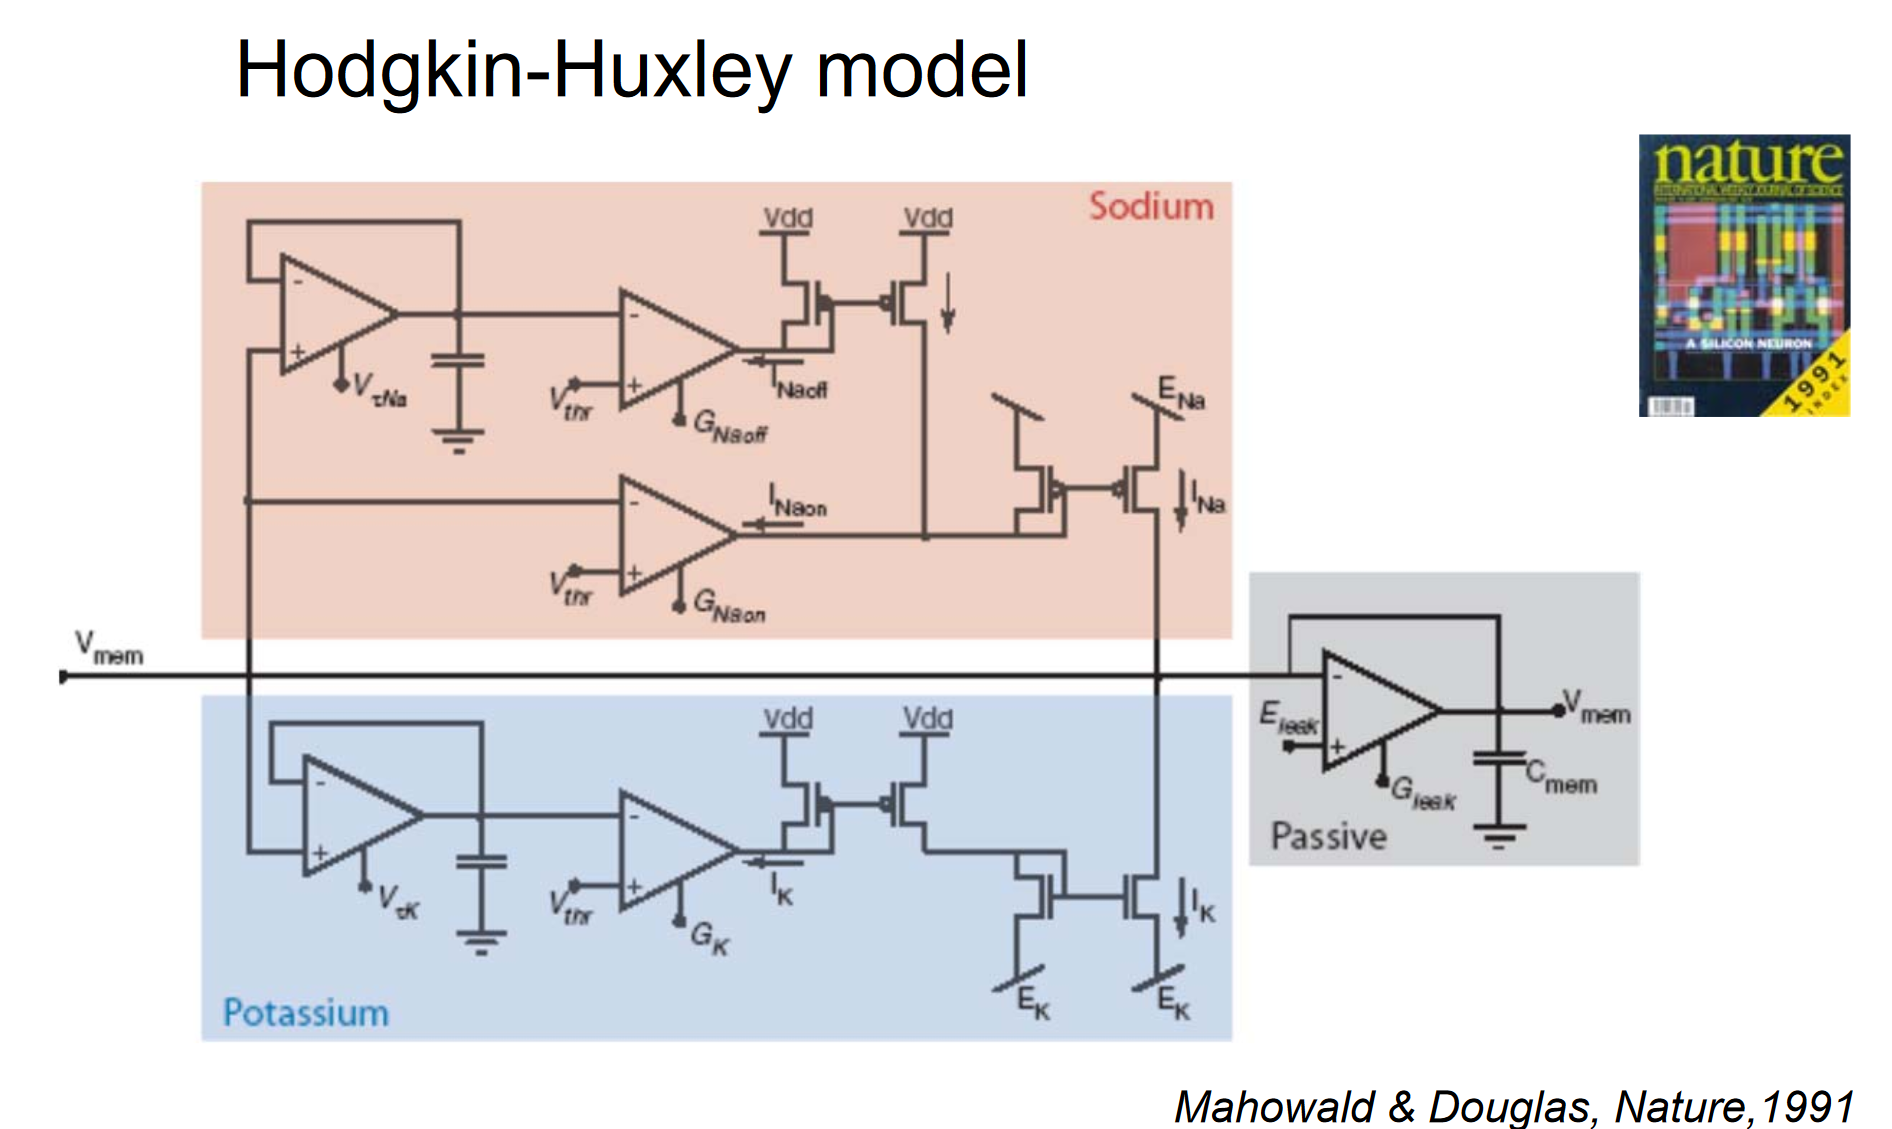
\includegraphics[width=0.8\linewidth]{11_NeuromorphicSystems1/figures/hh_model.png}
    \caption{A silicon neuron circuit.}
    \label{fig:hh}
\end{figure}
%

Processors harnessing both digital and analog techniques have been built in the past decade and they are presented in more detail in Lecture 12.

\subsection{Modelling vision and audition}
\subsubsection{Dynamic Vision Sensor: silicon retina}
The human retina contains around $10^8$ analog receptors, $10^6$ ganglion cells with spiking outputs and $10^9$ dynamic range modulating cells while consuming less than 3 mW of power. The retinal cone cells perform a special function of adjusting the operating point and the gain according to background illumination. This is driven by an active cell adaptation mechanism which is manifested as a shift in the light intensity-response curve, providing high sensitivity even in very low-light conditions. This property of the retina has inspired inventors in building state-of-the-art imaging sensors like the Pixel DVS, whose main components are depicted in Figure \ref{fig:dvs}.
%
\begin{figure}[h]
    \centering
    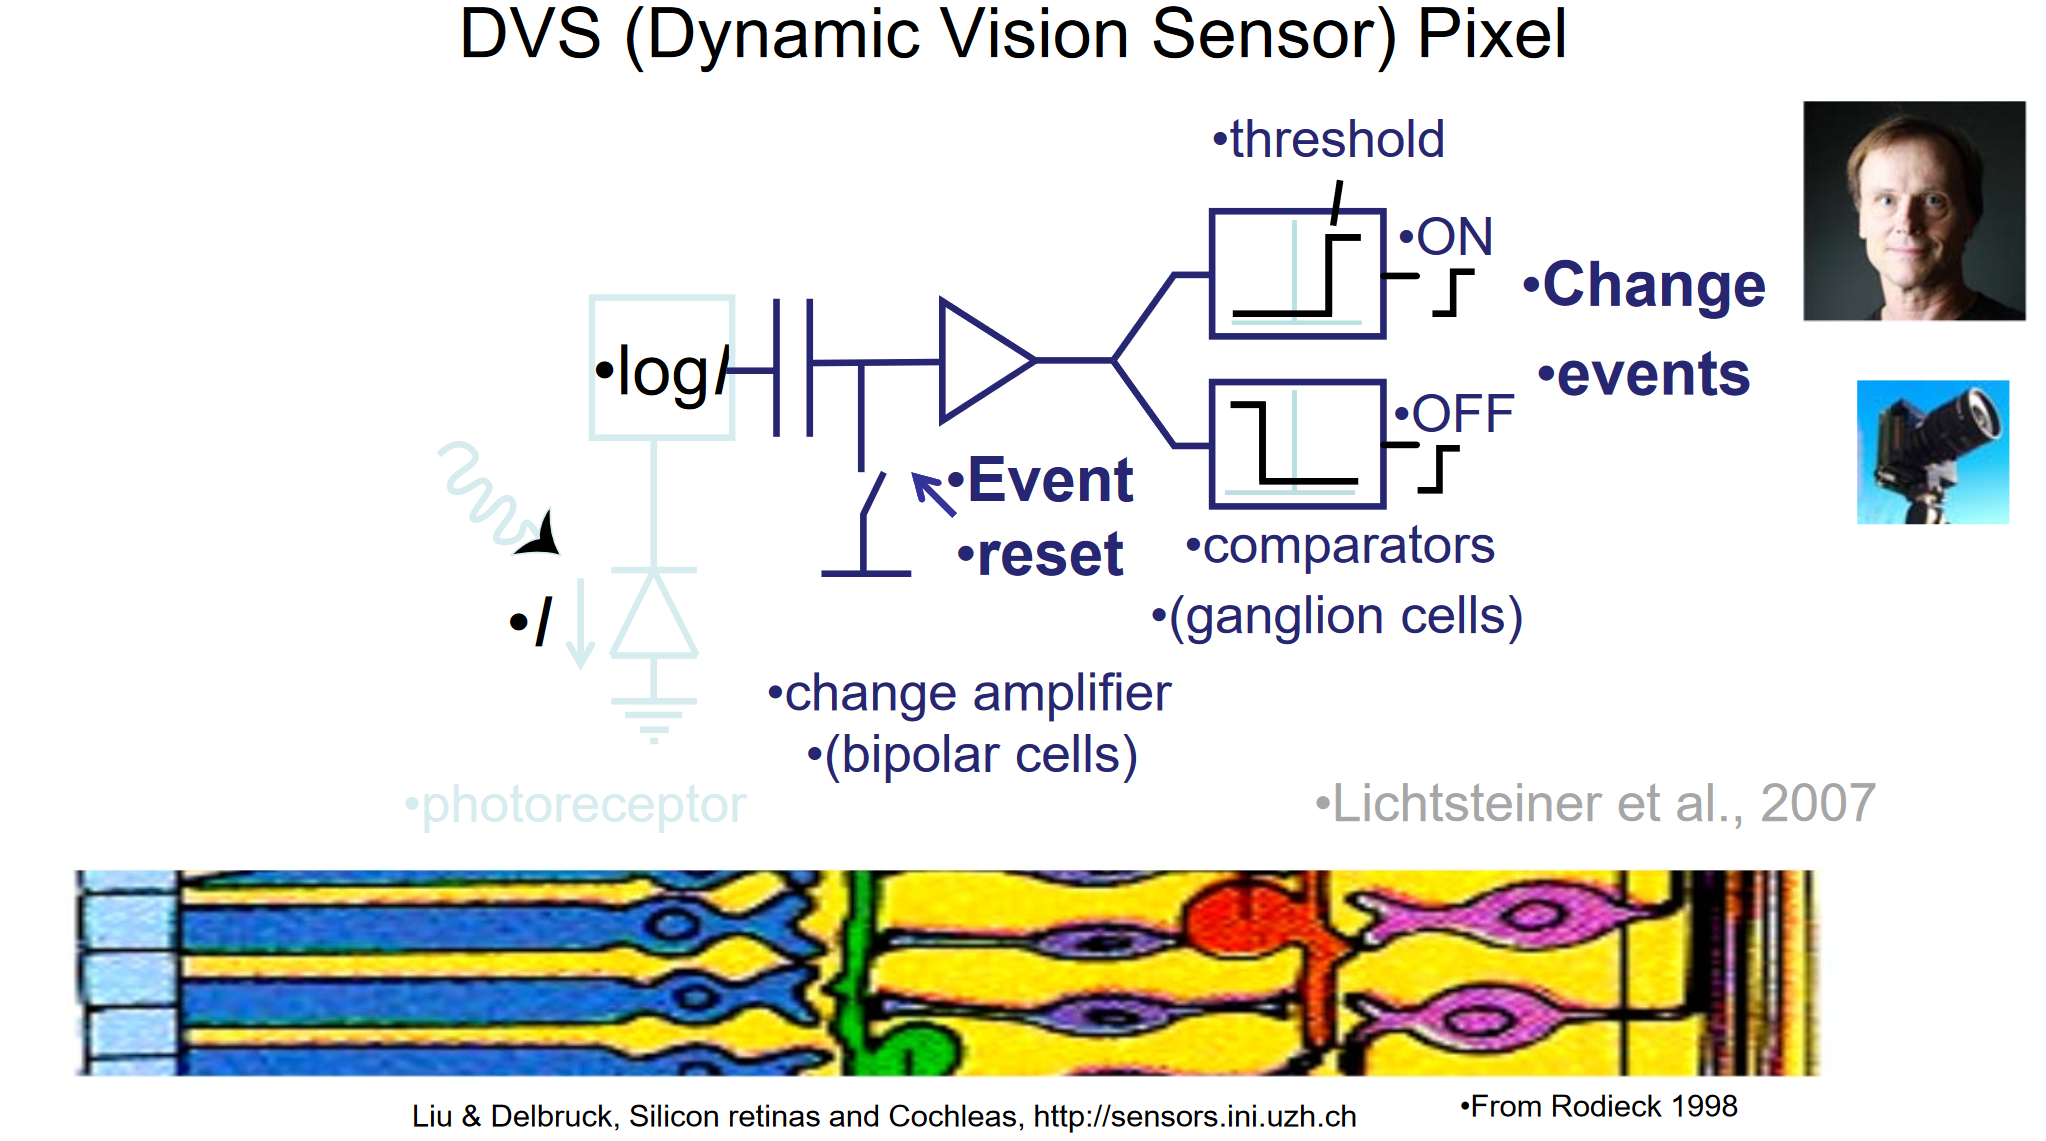
\includegraphics[width=0.8\linewidth]{11_NeuromorphicSystems1/figures/DVS.PNG}
    \caption{The Pixel Dynamic Vision Sensor.}
    \label{fig:dvs}
\end{figure}
%
The log-domain photoreceptor is the correspondent of the cone cell, the 
\subsubsection{Dynamic Audio Sensor: silicon cochlea}
\subsection{Sensors driving event-driven Deep Learning networks}
\subsubsection{Background of deep networks and biological aspirations}
\subsubsection{Spiking neurons + deep network systems}
\subsubsection{Data-driven deep networs}
\subsubsection{Conversion of deep ANN to deep SNN}

\end{document}